\documentclass[tikz,border=6pt]{standalone}
\usepackage{pgfplots}
\pgfplotsset{compat=1.18}
\begin{document}
% Data from simulator/run_simulator.py via paper/CAL/build/extract_sa_util.py
% Measured: QKV 41.3%, Attn 31.7%, FFN 40.5%, Dec1x1 28.3% (ViT-S DA2 encoder + DPT decoder, 518x518)
% Analytical: LiteMLA ours 71% / baseline 42% (1.7x FP32 side-path penalty);
%             Depthwise ours 78% / baseline 39% (2x GEMM-expansion penalty on banded weights).
% Baseline = ours for matmul-friendly phases (QKV / Attn / FFN / Dec1x1); differentiation shows on LiteMLA / Depthwise.
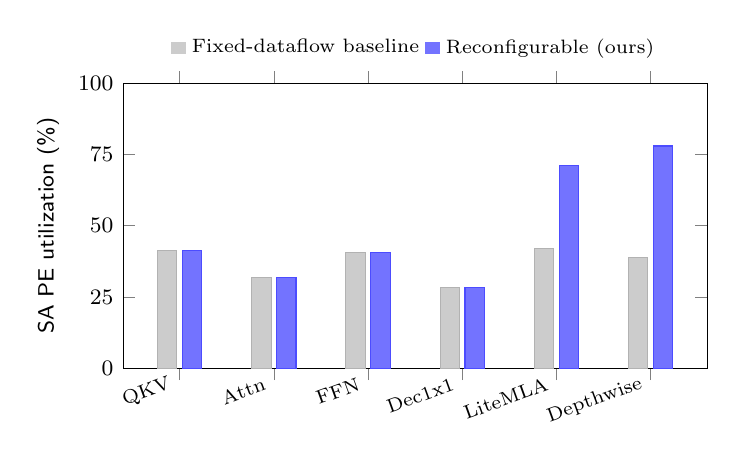
\begin{tikzpicture}
\begin{axis}[
  ybar=2pt,
  width=9cm,height=5.2cm,
  bar width=7pt,
  font=\sffamily\footnotesize,
  ylabel={SA PE utilization (\%)},
  ymin=0,ymax=100,
  ytick={0,25,50,75,100},
  symbolic x coords={QKV,Attn,FFN,Dec1x1,LiteMLA,Depthwise},
  xtick=data,
  x tick label style={rotate=20,anchor=east,font=\scriptsize},
  enlarge x limits=0.12,
  legend style={at={(0.5,1.05)},anchor=south,legend columns=-1,draw=none,font=\scriptsize},
  legend image code/.code={\draw[#1,draw=none] (0cm,-0.08cm) rectangle (0.2cm,0.08cm);},
  nodes near coords style={font=\tiny},
]
\addplot[fill=gray!40,draw=gray!60] coordinates {(QKV,41.3)(Attn,31.7)(FFN,40.5)(Dec1x1,28.3)(LiteMLA,42)(Depthwise,39)};
\addplot[fill=blue!55,draw=blue!70] coordinates {(QKV,41.3)(Attn,31.7)(FFN,40.5)(Dec1x1,28.3)(LiteMLA,71)(Depthwise,78)};
\legend{Fixed-dataflow baseline,Reconfigurable (ours)}
\end{axis}
\end{tikzpicture}
\end{document}
